\documentclass[a4paper, 12pt]{article}

\usepackage{hyperref}
\usepackage{fullpage}
\usepackage[top=1in, bottom=1.5in, left=1in, right=1in, footskip=4em]{geometry}
\usepackage{amsmath}
\usepackage{fancyhdr}
\usepackage[usenames,dvipsnames]{xcolor}
\usepackage{pgfornament}

\usepackage[shortlabels]{enumitem}
\usepackage{xspace}
\usepackage{lastpage}
\usepackage{multicol}
\usepackage{blindtext}
\usepackage{titling}
\usepackage{standalone}
\usepackage{amsfonts}
\usepackage[framemethod=TikZ]{mdframed}
\usetikzlibrary{calc}
\usepackage{lineno}
\usepackage{amsthm}
\usepackage{amssymb}
\usepackage{mathtools}
\usepackage{datetime}
\usepackage[most]{tcolorbox}
\usepackage{cancel}
\usepackage{ulem}
\usetikzlibrary{tikzmark, trees, backgrounds, graphs}
\usetikzlibrary{graphdrawing,graphs} 
\usetikzlibrary{decorations.markings}
\usetikzlibrary{decorations.pathmorphing, calc}
\usegdlibrary{layered, force}
\usepackage{pgfplots}
\linenumbers
\usepackage{tikz-qtree}

\setlength{\parskip}{1em}

%BEGIN_FOLD Commands
\usepackage{amssymb}% http://ctan.org/pkg/amssymb
\usepackage{pifont}% http://ctan.org/pkg/pifont
\newcommand{\cmark}{\ding{51}}%
\newcommand{\xmark}{\ding{55}}%
\newcommand{\half}{\ensuremath{\frac{1}{2}}}
\newcommand{\epv}[1]{\ensuremath{\left< #1 \right>}\xspace}
\newcommand{\variance}{\ensuremath{\text{Var}}}
\newcommand{\eout}{\ensuremath{E_\text{out}}\xspace}
\newcommand{\ein}{\ensuremath{E_\text{in}}\xspace}
\newcommand{\cx}{\ensuremath{\mathcal{X}}\xspace}
\newcommand{\cz}{\ensuremath{\mathcal{Z}}\xspace}
\newcommand{\real}{\mathbb{R}}
\DeclareSymbolFont{extraup}{U}{zavm}{m}{n}
\DeclareMathSymbol{\varheart}{\mathalpha}{extraup}{86}
\DeclareMathSymbol{\vardiamond}{\mathalpha}{extraup}{87}
\renewcommand{\heartsuit}{\textcolor{red}{\varheart}}
\renewcommand{\diamondsuit}{\textcolor{red}{\vardiamond}}
\newcommand{\definition}{\vspace{1em}\noindent\textbf{Def:} }
\newcommand{\theorem}{\vspace{1em}\noindent\textbf{Theorem:} }
\newcommand{\collorary}{\vspace{1em}\noindent\textbf{Theorem:} }
\newcommand{\example}{\vspace{1em}\noindent\textbf{Example:} }
\newcommand{\solution}{\newline\noindent\textbf{Solution:} }
\newcommand{\predicate}{\vspace{0.25em}\noindent\textbf{Inductive Predicate:} }
\newcommand{\inductivestep}{\vspace{0.25em}\noindent\textbf{Inductive Step:} }
\renewcommand{\proof}{\vspace{0.5em}\noindent\textbf{Proof:} }
\newcommand{\lemma}{\vspace{1em}\noindent\textbf{Lemma:} }
\newcommand{\hint}{\textbf{Hint:} }
\newcommand{\basecase}{\vspace{0.25em}\noindent\textbf{Base Case:} }
\newcommand{\inductivehypothesis}{\vspace{0.25em}\noindent\textbf{Inductive Hypothesis:} }
\renewcommand{\collorary}{\vspace{1em}\noindent\textbf{Collorary:} }
\newcommand{\qedd}{\qed\newline}
\newcommand{\kwd}[1]{\textcolor{blue}{\textbf{\underline{#1}}}}
\newcommand\ColorBox[2][]{%
	\stepcounter{mybox}%
	\node[draw=red!70!black,fill=red!20,align=left,#1] (box\themybox) {#2};
}
\newcommand{\expl}[2]{%
	\underset{\substack{\uparrow\\\mathrlap{\text{\hspace{-1em}#2}}}}{#1}}
\newcommand{\uexpl}[2]{%
	\overset{\substack{\mathrlap{\text{\hspace{-1em}#2}}\\\downarrow}}{#1}}
\newcommand{\st}{\text{ such that }}
\newcommand{\R}{\textcolor{red}{R}}
\newcommand{\sumn}{\sum^n_{i=0}}
\newcommand{\sumxn}{\sum^n_{x=0}}
\newcommand{\red}[1]{\textcolor{red}{#1}}
\newcommand{\blue}[1]{\textcolor{blue}{#1}}

%\newcommand{\qed}{\ensuremath{\blacksquare}}
%END_FOLD
\newcommand{\sidenote}[1]{\textcolor{gray}{#1}}
\let\Pr\relax
\DeclareMathOperator{\Pr}{Pr}
\DeclareMathOperator{\E}{\mathbb{E}}
\DeclareMathOperator{\Cov}{Cov}
%BEGIN_FOLD miscellaneious default
\makeatletter
% Make a copy of macros responsible for entering display math mode
\let\start@align@nopar\start@align
\let\start@gather@nopar\start@gather
\let\start@multline@nopar\start@multline
% Add the "empty line" command to the macros
\long\def\start@align{\par\start@align@nopar}
\long\def\start@gather{\par\start@gather@nopar}
\long\def\start@multline{\par\start@multline@nopar}
\makeatother
\setlength{\columnsep}{1cm}
%opening
\setlength{\abovedisplayskip}{-\baselineskip}%
\setlength{\abovedisplayshortskip}{\abovedisplayskip}%

\pagestyle{fancy}
\renewcommand{\headrulewidth}{0pt}
\lfoot{\small{\course}: Week \weekno}
\rfoot{\small{\thetitle}}
\rhead{}
\cfoot{\pgfornament[height=1em, ydelta=-0.4em]{17} \thepage of \pageref{LastPage}  \pgfornament[height=1em, ydelta=-0.4em]{18}}

\DeclareMathOperator{\sign}{sign}
\DeclareMathOperator{\Var}{Var}
\newcommand{\vect}[1]{\ensuremath{\mathbf{#1}}\xspace}

\tikzstyle{every picture}+=[remember picture]
\newcommand{\bwgrid}[1]{
	\def \aaa #1
	
	\foreach \y in {0,1,2} {
		\foreach \x in {0,1,2} {
			\pgfmathsetmacro{\clr}{\aaa[\x][\y]}
			%\message{aaa \clr}
			\definecolor{MyColor}{rgb}{\clr,\clr,\clr}
			\path[fill=MyColor] (\x,\y) rectangle ++(1,1); 
		}
	}
	\draw[step=1cm,very thin] (0,0) grid (3,3);	
}

\setenumerate{label=\alph*.)}
\definecolor{db}{RGB}{100,65,23}

%END_FOLD
\definecolor{land}{HTML}{95EA64}
\definecolor{water}{HTML}{BBE0E3}
\definecolor{bridge}{HTML}{FEFF9E}
\newcommand{\course}{Discrete Math}
\title{Graph Theory}
\newcommand{\weekno}{11}

\begin{document}
\begin{center}
	\textcolor{orange}{\textsc{\course}}\\
	\huge\textbf{\textsc{\thetitle}}\\
	\small\textcolor{gray}{Last updated:\, \today \, \currenttime}\\
	\pgfornament[width=0.7\textwidth, color=white!30!black]{88}
\end{center}



	
	Let us consider the problem of whether, on average, male has more female facebook friends or female has more average male friends on facebook. This seems to be a good measure of how each sex is more popular than the other.
	
	The relationship between male and female on facebook can be represented with nodes representing users and the line connecting the users represent whether they are friends or not.
	
\begin{center}
		\begin{tikzpicture}[male/.style={circle, draw, fill=blue!20!white}, female/.style={circle, draw, fill=red!20!white}]
		\node (m1)[male] {};
		\node (m2)[below of=m1, male] {};
		\node (m3)[below of=m2, male] {};
		\node (m4)[below of=m3, male] {};
		
		\node (g1)[right of=m1, xshift=2cm, female] {};
		\node (g2)[below of=g1, female] {};
		\node (g3)[below of=g2, female] {};
		
		\draw (m1) -- (g1);
		\draw (m2) -- (g1);
		\draw (m3) -- (g2);
		\draw (m3) -- (g3);
		\draw (m3) -- (g1);
		\draw (m4) -- (g3);
		\draw (m1) -- (g3);
		
		\draw[dashed] (1.5,0.5) -- (1.5,-3);

	\end{tikzpicture}
\end{center}

	So, if we need to know the average number of female friends for a male user, then all we need to do is find total number of female friend male users has. This is just the number of edges(lines). So the average of opposite is
	\begin{center}
		Male Popularity = $\displaystyle \frac{\text{\# of edges}}{\text{\# of male}}$
	\end{center}
	
	Similarly, the average male friend for female users is given by
	\begin{center}
		Female Popularity = $\displaystyle \frac{\text{\# of edges}}{\text{\# of female}}$
	\end{center}	

	The ratio of the two, in fact, has nothing about how popular each sex is on average. It just has to do with the total number of each sex in the population.
	\begin{center}
		$\displaystyle \frac{\text{Male Popularity}}{\text{Female Popularity}} =  \frac{\text{\# of female}}{\text{\# of male}}$
	\end{center}
	
	\section*{Graph}
	In the former example, we can see that the problem becomes much clearer if we strat drawing doodles representing objects of interest and the relation among them. Since the doodle has so many uses it has a fancy name called graph.
	
	\definition A simple graph $G$ consists of non-empty set $V$, called vertices or nodes of $G$ and a set $E$ of two element subset of $V$. The member of $E$ are called edges of $G$. We write $G= (V,E)$.
	
	For example, the following graph
	\begin{center}
			\begin{tikzpicture}[spring layout, every node/.style={circle, draw, minimum size=1cm}]
			\begin{graph}[layered layout, sibling distance=1cm, level distance=1cm]
			{
				a -- {c,b} -- d;
				b--e;
				b--f;
			};
			\end{graph}
		\end{tikzpicture}
	\end{center}
	
	The vertex are
	\[
		V = \{a, b, c, d, e\}.
	\]
	The edges are
	\[
		E = \{ (a,b), (a,c), (c,d), (b,d), (b,e), (b,f)\}.
	\]
	
	
	\definition Two vertices of in a simple graph are \emph{adjacent} if there is an edge connect the two.
	
	\definition An edge is said to be \emph{incident} to the vetices it joins.
	
	\definition The number of edges incident to the node is called the \emph{degree} of the vertex.
	
	For example, a complete graph of $n$ vertices has $\displaystyle {n \choose 2} edges$. The figure below shows a complete graph of $5$ vertices, $K_5$.
	\begin{center}
		\begin{tikzpicture}[spring layout, every node/.style={circle, draw, minimum size=1cm}]
		\begin{graph}[spring layout, sibling distance=1cm, level distance=1cm]
		{
			a -- {b, c, d, e};
			b -- {c, d, e};
			c -- {d, e};
			d -- e;
		};
		\end{graph}
		\end{tikzpicture}
	\end{center}
	
	\section*{Isomorphism}
	
	\definition If $G_1 = (V_1, E_1)$ and $G_2 = (V_2, E_2)$ then $G_1$ is \emph{isomorphic} to $G_2$ iff there exists a bijection $f: V_1 \to V_2$ such that for all pair $u,v \in V_1$
	\[
		\{u, v\} \in E_1 \text{ iff } \{f(u), f(v)\} \in E_2
	\]
	The bjection $f$ is called an \emph{isomorphism} between $G_1$ and $G_2$.
	
	In simple words, $G_1$ and $G_2$ are isomorphic if they are the same graph up to relabeling. For example, the two graphs below are isomorphic. 
	\begin{center}
			\begin{tikzpicture}[every node/.style={draw,circle, minimum size=1cm}]
			\begin{scope}[xshift = 2cm]
				\node (A) at (0:2cm) {A};
				\node (B) at (72:2cm) {B};
				\node (C) at (144:2cm) {C};
				\node (D) at (216:2cm) {D};
				\node (E) at (288:2cm) {E};
				
				\draw (A) edge (B) (B) edge (C) 
					(C) edge (D) (D) edge (E)
					(E) edge (A);
			\end{scope}
			
			\begin{scope}[xshift = 8cm]
				\node (n1) at (0:2cm) {1};
				\node (n2) at (72:2cm) {2};
				\node (n3) at (144:2cm) {3};
				\node (n4) at (216:2cm) {4};
				\node (n5) at (288:2cm) {5};
				\draw (n1) edge (n3) (n3) edge (n5) (n5) edge (n2)
				(n2) edge (n4) (n4) edge (n1);
			\end{scope}
			
		\end{tikzpicture}
	\end{center}
	The isomorphism is
	\[
		1 \to A, 3 \to B, 5 \to C, 2 \to D, 4 \to E 
	\]
	
	\section*{Subgraph}
	
	\definition A graph $G_1 = (V_1, E_1)$ is a \emph{subgraph} of $G_2 = (V_2, E_2)$ if $V_1 \subseteq V_2$ and $E_1 \subseteq E_2$. We write $G_1 \subseteq G_2$.
	
	For example,
	\begin{center}
			\begin{tikzpicture}[every node/.style={draw,circle, minimum size=1cm}]
			
				\begin{scope}[]
				\node (A) at (0:2cm) {A};
				\node (B) at (72:2cm) {B};
				%\node (C) at (144:2cm) {C};
				\node (D) at (216:2cm) {D};
				\node (E) at (288:2cm) {E};
				
				\draw (A) edge (B) 
	 (D) edge (E);
				\end{scope}
				
				\node[draw=none] at (4,0) {$\subseteq$};
			
				\begin{scope}[xshift = 7cm]
				\node (A) at (0:2cm) {A};
				\node (B) at (72:2cm) {B};
				\node (C) at (144:2cm) {C};
				\node (D) at (216:2cm) {D};
				\node (E) at (288:2cm) {E};
				
				\draw (A) edge (B) (B) edge (C) 
				(C) edge (D) (D) edge (E)
				(E) edge (A);
				\end{scope}
			\end{tikzpicture}
	\end{center}
	
	\section*{Handshaking Lemma}
	
	\lemma The sum of degree is $2|E|$.
	
	\proof Every edge contribute two to the sum of the degree. 
	\qed
	
	\collorary In any graph there are even number of vertices of odd degree.
	
	\proof Otherwise the total number of degree would be odd.
	\qed
	
	\section*{Coloring}
	
	Let us consider the problem of assigning exam to timeslot. We do not want to have two exams on the same time slot.
	
	Let us draw a graph for this. Let the node represent the class and the edge represent whether there is any student taking the two classes. Let suppose the graph for our classes look like this
	
\begin{center}
		\begin{tikzpicture}[every node/.style={circle, draw, minimum size=1cm}, node distance=2cm]
	
	\node(a) {};
	\node[below left of=a](b) {};
	\node[below right of=a](c) {};
	\node[below left of=c](d) {};
	\node[right of=d](e) {};
	\node[above right of=e](f) {};
	\node[below right of=e](g) {};
	
	\draw (a) edge (b) (a) edge(c);
	\draw (b) edge (d) (b) edge (c);
	\draw (c) edge (d);
	\draw (d) edge (e);
	\draw (e) edge (f) (e) edge (g);
	\end{tikzpicture}
\end{center}

	Suppose that you have couple time slot of the exams, A:8-10am, B:10-12pm, C:12-2pm, D:2-4pm, E:4-6pm. 
	
	One obvious solution is to give each of the class their own time slot. But, no one wants to take exam in the late evening. So we want to use as least timeslots as possible. On the other hand, if we don't have enough time slot there will be time conflict between some exams.

	The problem we have here is to assign the timeslot(color) to the class(node) such that no two adjacent node has the same color. This is called coloring problem. Here are some possible assignments.

	
	\begin{center}
			\begin{tikzpicture}[every node/.style={circle, draw, minimum size=1cm}, node distance=2cm,
			fg/.style={fill=green!20!white},
			fr/.style={fill=red!20!white},
			fb/.style={fill=blue!20!white},
			fm/.style={fill=magenta!20!white}]
			\begin{scope}
				\node[fb](a) {B};
				\node[below left of=a, fg](b) {A};
				\node[below right of=a,fm](c) {D};
				\node[below left of=c,fr](d) {C};
				\node[right of=d,fb](e) {B};
				\node[above right of=e, fg](f) {A};
				\node[below right of=e,fr](g) {C};
				
				\draw (a) edge (b) (a) edge(c);
				\draw (b) edge (d) (b) edge (c);
				\draw (c) edge (d);
				\draw (d) edge (e);
				\draw (e) edge (f) (e) edge (g);
			\end{scope}
			
			\begin{scope}[xshift=7cm]
				\node[fg](a) {A};
				\node[below left of=a, fb](b) {B};
				\node[below right of=a, fr](c) {C};
				\node[below left of=c, fg](d) {A};
				\node[right of=d, fb](e) {B};
				\node[above right of=e, fg](f) {A};
				\node[below right of=e, fr](g) {C};
				
				\draw (a) edge (b) (a) edge(c);
				\draw (b) edge (d) (b) edge (c);
				\draw (c) edge (d);
				\draw (d) edge (e);
				\draw (e) edge (f) (e) edge (g);
			\end{scope}
		\end{tikzpicture}
	\end{center}
	
	Both of the graph above are valid coloring scheme. But, they do not use the same number of color. The minimum number of color needed to color a graph is called the chromatic number.
	
	\definition The minimum number of color needed to color a graph $G$ is called \emph{chromatic number}. $\chi(G)$
	
	Trying to figure out the chromatic number for a gerneral graph is an NP complete problem (which means the best way to solve it as far as we know is non polynomial time.).
	
	That being said it is quite easy to find a valid coloring (not necessarily optimal) scheme. Let us consider a greedy algorithm.
	
	\begin{itemize}
		\item First, we order the vertices (doesn't matter how).\[
			v_1, v_2, v_3 , \ldots, v_n
		\]
		\item We then order the color
		\[
			c_1, c_2, c_3, \ldots, c_m
		\]
		\item Go through each vertex in the list give it the lowest color.
	\end{itemize}
	
	%Insert picture here
	
	We can also bound the 
	
	\theorem A graph with a maximum of $d$ degree is $d+1$ colorable.
	
	\proof We will do this by induction. Miss it? For induction on graph always try to induct on number of node or edges. Never ever do induction on the number of degree.
	
	\predicate $P(s)$:= Graph of $s$ nodes with maximum degree of $d$ is $d+1$ colorable for all positive integer $d$.
	
	\basecase Graph of 1 node has 0 degree and is 1 colorable.
	
	\inductivestep The strategy here is to take away one node so we have a smaller graph we will then add it back.
	\begin{itemize}
	\item Let us assume that any graph of $k$ node with maximum degree of $d$ is $d+1$ colorable for all $d$.
	
	\item Let us consider a graph of $k+1$ node with maximum degree of $d$.


	\begin{center}
				\begin{tikzpicture}[every node/.style={circle, draw, minimum size=1cm}]
					\node (A) at (0:2cm) {A};
					\node (B) at (72:2cm) {B};
					\node (C) at (144:2cm) {C};
					\node (D) at (216:2cm) {D};
					\node (E) at (288:2cm) {E};
					\draw (0,0) circle (3cm) node[below, draw=none,yshift=-3cm, rectangle]{$k$ nodes with maximum of $d$ degree.};
					\node (F) at (7cm,0) {F};
					\draw[dashed] (F) -- (B) (F)--(C) (F)--(D);
					\node[draw=none, yshift=+1cm] at ($(0,0)!0.7!(F)$) {maximum of $d$ edges};
			\end{tikzpicture}
	\end{center}


	\item We can split it into
	\begin{enumerate}
		\item A subgraph of $k$ nodes and the maximum degree $d$. By inductive hypothesis, we know that this subgraph need at most $d+1$ color.
		\item A node $F$.
	\end{enumerate}
	
	\item  Since the degree of $F$ is at most $d$, the number of edge linking $F$ back to the subgraph is at most $d$.
	
	\item The subgraph use $d+1$ color and there are at most $d$ edges link $F$ with the subgraph. There is at least 1 color from $d+1$ color that is not used by any node connected to $F$.
	
	\item We can use that color to color $F$. We do not need extra color for $F$. So, the total color needed is $d+1$ for the subgraph.
	
	\end{itemize}
	\qed
	
	
	It should be noted that this may give you an unnecessary large upper bound. Let us consider a graph that looks like the following
	
	\begin{center}
		\begin{tikzpicture}[every node/.style={draw, circle, minimum size=1cm}]
			\node (A) at (0:2cm) {A};
			\node (B) at (72:2cm) {B};
			\node (C) at (144:2cm) {C};
			\node (D) at (216:2cm) {D};
			\node (E) at (288:2cm) {E};
			\node (F) at (0,0) {F};
			
			\draw (F)--(A) (F)--(B) (F)--(C) (F)--(D) (F)--(E); 	
		\end{tikzpicture}
	\end{center}
	
	Even though you only need two color for the above graph. The bound we proves says that we need 6 color to do it.
	
	\subsection*{When the Algorithm does not do well}
	
	There are certain case where the algorithm does not do too well. If we have a graph that looks like the following:
	\begin{center}
			\begin{tikzpicture}[every node/.style={draw, circle, minimum size=1cm}, node distance=2cm]
			\node (A) {A};
			\node[below of=A] (B) {B};
			\node[below of=B] (C) {C};
			
			\node[right of=A , xshift=+2cm] (D) {D};
			\node[below of=D] (E) {E};
			\node[below of=E] (F) {F};
			
			%\draw (A) -- (D);
			\draw (A) -- (E);
			\draw (A) -- (F);
			
			\draw (B) -- (D);
			%\draw (B) -- (E);
			\draw (B) -- (F);
			
			\draw (C) -- (D);
			\draw (C) -- (E);
			%\draw (C) -- (F);
		\end{tikzpicture}
	\end{center}
	If we order the vertices such that we order it like
	\[
		A,D,B,E,C,D
	\]
	then after you assign $c_1$ to $A$ then you will also assign $c_1$ to $D$. $c_2$ will be assigned to $B$ and $E$. Then $c_3$ will be assign to $C$ and $F$ and so on. We will need $|V|/2$ color instead of just 2 colors.
	
	%\subsection*{Traffic Control}
	
	\subsection*{Cell Tower Placement}
	
	Coloring problem is far more reaching than just mathematical play toy. Let us consider the problem of placing cell tower. Each cell tower has some range. But there is an annoying physics part that if two cell tower are in range of each other, we cannot use the same frequency since they will interfere. So, for the two cell towers that has overlapping area we need to assign different frequencies to each tower.
	
	\subsection*{Art Museum Theorem}
	
	Let us consider the problem of guarding an art museum. Let us assume that art museum is a simple polygon(no hole). We need to place guards such that we cover the whole museum. One way to do it is to place the guard at every single corners but that would be overkill. The cost for security guard will run too high. So we need to figure out the way to find smaller number of guards.
	
	\begin{center}
			\begin{tikzpicture}
			%\draw[step=0.5cm] (0,0) grid (6,6);
			\coordinate (A) at (2.5,2);
			\coordinate (B) at (1,1);
			\coordinate (C) at (2,3);
			\coordinate (D) at (0,4);
			\coordinate (E) at (3,6);
			\coordinate (F) at (2,5);
			\coordinate (G) at (4,4);
			\coordinate (H) at (3,0);
			\draw (A) -- (B) -- (C) -- (D) -- (E) -- (F) --(G) -- (H) --cycle;
		\end{tikzpicture}
	\end{center}
	
	Let us triangulate the museum. The idea is that to cover a triangle all we need to do is place a guard at one of the corner then the triangle is covered. We will prove later that triangulation is always possible.
	
	\begin{center}
		\begin{tikzpicture}
		%\draw[step=0.5cm] (0,0) grid (6,6);
		\coordinate (A) at (2.5,2);
		\coordinate (B) at (1,1);
		\coordinate (C) at (2,3);
		\coordinate (D) at (0,4);
		\coordinate (E) at (3,6);
		\coordinate (F) at (2,5);
		\coordinate (G) at (4,4);
		\coordinate (H) at (3,0);
		
%		\node at (A) {A};
%		\node at (B) {B};
%		\node at (C) {C};
%		\node at (D) {D};
%		\node at (E) {E};
%		\node at (F) {F};
%		\node at (G) {G};
%		\node at (H) {H};
		
		\draw (A) -- (B) -- (C) -- (D) -- (E) -- (F) --(G) -- (H) --cycle;
		\draw (A) -- (C) (C) -- (G) (A) -- (G) (C) -- (F) (D) -- (F); 
		\end{tikzpicture}
	\end{center}
	
	That means all we need to do now is to color the nodes. Each color represent each set of different placement of guard. We don't want the same set of guard to be guarding the same triangle since that would be a waste of money. To do this we only need 3 colors.
	
	\begin{center}
		\begin{tikzpicture}[r/.style={fill=red!50!white, minimum size=0.5cm,circle},
		g/.style={fill=green!50!white, minimum size=0.5cm,circle},
		b/.style={fill=blue!50!white, minimum size=0.5cm,circle}]
		%\draw[step=0.5cm] (0,0) grid (6,6);
		\coordinate (A) at (2.5,2);
		\coordinate (B) at (1,1);
		\coordinate (C) at (2,3);
		\coordinate (D) at (0,4);
		\coordinate (E) at (3,6);
		\coordinate (F) at (2,5);
		\coordinate (G) at (4,4);
		\coordinate (H) at (3,0);
		
		\node[r] at (A) {};
		\node[b] at (B) {};
		\node[g] at (C) {};
		\node[b] at (D) {};
		\node[g] at (E) {};
		\node[r] at (F) {};
		\node[b] at (G) {};
		\node[g] at (H) {};
		
		\draw (A) -- (B) -- (C) -- (D) -- (E) -- (F) --(G) -- (H) --cycle;
		\draw (A) -- (C) (C) -- (G) (A) -- (G) (C) -- (F) (D) -- (F); 
		\end{tikzpicture}
			\end{center}
		For the example above we have 2 red, 3 blue and 3 green. That means if we place the guards at 3 blue vertiecs we will cover all the regions. Or we can place just 2 guards at the 2 red vertices then we have every thing covered. Let $n$ be the number of vertices and $r$ be number of red vertex, $b$ for the number of blue vertex, and $g$ for the number of green vertex. Then we have
		\[
			r + g + b = n
		\]
		
		This means that there is at least one of the color with less or equal to $n/3$. Otherwise the sum will be greater than $n$.
		
		The result is called Art Muesum Theorem saying the minimum number of guard needed to guard $n$ vertex simple polygon is at most $n/3$. This elegant prove is by Steve Frisk while dozing off a bus in Afganistan.\footnote{\url{http://bowdoinorient.com/article/4980}}

		Now let us fill in the missing holes.
	
	
	\subsubsection*{Triagulation is Always Possible}
	
	\theorem Given a polygon triangulation is always possible.
	
	\proof We will show this by induction on the number of vertex. You can fill in the formality.
	
	If we have a triangle then it is trivial to triangulate. It is already a triangle. There is nothing to do here.
	
	Let us consider an $n$ vertex polygon. The consider three adjacent vertices $v$, $u$ and $w$. There are two cases for the three vertices.
	\begin{enumerate}
		\item If the triangle form by the three vertices has no node inside then we have a triangle and an $n-1$ vertices polygon. We know we can triangulate both by inductive hypothesis. 
		\begin{center}
			\begin{tikzpicture}
				%\draw[step=0.5cm] (0,0) grid (6,6);
				\coordinate (A) at (2.5,2);
				\coordinate (B) at (1,1);
				\coordinate (C) at (2,3);
				\coordinate (D) at (0,4);
				\coordinate (E) at (3,6);
				\coordinate (F) at (2,5);
				\coordinate (G) at (4,4);
				\coordinate (H) at (3,0);
				\draw (A) -- (B) -- (C) -- (D) -- (E) -- (F) --(G) -- (H) --cycle;
				\node[above] at (A) {u};
				\node[left] at (B) {v};
				\node[above] at (C) {w};

				\draw [dashed] (A) -- (C);
			\end{tikzpicture}%inser figure here
		\end{center}

		\item If the triangle formed by $u$, $v$ and $w$ has some vertices inside. Then, all we need to do is pick the vertex that is closest\footnote{closest here means the distance between the line parallel to $\overline{uw}$ that pass through that point is closets to $v$} to $v$ that is not $u$ or $w$. let us call that point $p$. 
		
		The reason that we pick such a line is because the line from $v$ to $p$ cut the polygon in to two smaller polygons\footnote{If it has a hole then all we need to do is keep cutting it if it doesn't split. The number of hole is finite and each time if we don't split the polygon we will destroy a hole. We guarantee to destroy all holes.} which we know can be triangulated.
			\begin{center}
				\begin{tikzpicture}[extended line/.style={shorten >=-#1,shorten <=-#1, red, thick},
				extended line/.default=1cm]
				%\draw[step=0.5cm] (0,0) grid (6,6);
				\coordinate (A) at (2.5,2);
				\coordinate (B) at (1,1);
				\coordinate (C) at (2,4);
				\coordinate (D) at (0,4);
				\coordinate (E) at (3,6);
				\coordinate (F) at (2,5);
				\coordinate (G) at (4,4);
				\coordinate (GG) at (2,3);
				\coordinate (GG2) at (2,2);
				\coordinate (GGG)  at(5,4);

				\coordinate (H) at (3,0);
				\draw (A) -- (B) -- (C) -- (D) -- (E) -- (F) --(G) -- (GG) -- (GG2) -- (GGG) -- (H) --cycle;
				\node[above] at (A) {u};
				\node[left] at (B) {v};
				\node[above] at (C) {w};
				\node[left] at (GG2) {p};
				\fill [gray, opacity=0.2] (A) -- (B) -- (C);
				\draw[dashed] (B) -- (GG2);
				\draw[dotted, extended line=0.5cm] (A) -- (C);
				\draw[dotted,extended line=0.5cm] (GG) -- +($(A)-(C)$);
				\draw[dotted,extended line=0.5cm] (GG2) -- +($(A)-(C)$);
				\end{tikzpicture}%inser figure here
			\end{center} 
	\end{enumerate}
	\qedd
	

	\subsubsection*{Two ears theorem}
	\theorem Every simplex polygon with $n\ge 4$ has at least two ears. An ear is a three adjacent vertices that form a diagonal line(no other vertex in the triangle).
	
	\proof We can proof by the same construct as the previous problem by picking three vertices.
	
	The base case is a square. That's trivial.
	
	Let us consider simple polygon with $n>5$
	
	\begin{enumerate}
		\item If $u$, $v$ and $w$ form an ear, then we end up with an ear and a smaller polygon with 2 ears by IH. When we combine them back since they share at most 1 edge(no hole), we can destroy at most 1 ear if that edge belongs to an ear of the left over polygon. So the number of left over ear is still $\ge 2$.
		
		\item If $u$, $v$ and $w$ does not form an ear, we again pick a point $p$ ``closest'' to the $v$ and cut the polygon into two. There are two cases.
		\begin{enumerate}
			\item One of them is triangle. Then we are back the previous case. Adding a triangle reduce the nubmer of edge. 
			\item If none of it is a triangle. Then you get two from both sides and you destroy at most two for the edge that we share.
			\item Ending up with 2 triangles is not possible since $n\ge 5$ 
		\end{enumerate}
	\end{enumerate}
	
	\subsubsection*{3 Color Theorem}
	\theorem Every triangulated graph of a simple polygon is 3 colorable. (No hole)
	
	\proof We will show this by induction on the number of triangles.
	
	The graph with 1 triangle is trivial to do.
	
	Let us consider a graph of $n$ triangles and let us remove one ear. The graph without that ear is 3 colorable by IH. Then all we need to do at add an ear back is to add a vertex. Since this vertex has exactly 2 edge. We can color this vertex with the left over color.
	\qedd
	
	\section*{Path Walk Connectivity}
	
	\definition A \emph{walk} is a sequence of vertices that are connected by edges. For example, the path
	\[
		v_1, v_3, v_2, v_6, v_3, v_7, v_8
	\]
	
	\begin{center}
			\begin{tikzpicture}[every node/.style={circle, draw, minimum size = 0.3cm}, scale =0.5]
		%\draw[] (0,0) grid (5,5);
		\node(v1) at (0,3) {$v_1$};
		\node(v2) at (3,0) {$v_2$};
		\node(v3) at (3,3) {$v_3$};
		\node(v4) at (3,6) {$v_4$};
		\node(v5) at (6,0) {$v_5$};
		\node(v6) at (6,3) {$v_6$};
		\node(v7) at (6,6) {$v_7$};
		\node(v8) at (9,3) {$v_8$};
		\draw (v1) -- (v2) (v1) -- (v3) (v1) -- (v4);
		\draw (v2) -- (v3);
		\draw (v4) -- (v7) (v4) -- (v6);
		\draw (v3) -- (v5) (v3) -- (v6) (v3) -- (v7);
		\draw (v2) -- (v5) (v2) -- (v6);
		\draw (v8) -- (v7) (v8) -- (v6) (v8) -- (v5);
		\begin{scope}[very thick,decoration={
			markings,
			mark=at position 0.5 with {\arrow{>}}}
		] 
		\draw[postaction={decorate}, red, ultra thick] (v1) -- (v3);
		\draw[postaction={decorate}, red, ultra thick] (v3) -- (v2);
		\draw[postaction={decorate}, red, ultra thick] (v2)-- (v6);
		\draw[postaction={decorate}, red, ultra thick] (v6) -- (v3);
		\draw[postaction={decorate}, red, ultra thick] (v3) -- (v7);
		\draw[postaction={decorate}, red, ultra thick] (v7) -- (v8);
		\end{scope}
		\end{tikzpicture}
	\end{center}
	
	
	\definition A \emph{path} is a walk where all the vertices are different. So the walk we gave in the earlier example is not a path. Here is an example of a path
	\[
		v_1, v_3, v_7, v_8
	\]
	
	\begin{center}
		\begin{tikzpicture}[every node/.style={circle, draw, minimum size = 0.3cm}, scale =0.5]
		%\draw[] (0,0) grid (5,5);
		\node(v1) at (0,3) {$v_1$};
		\node(v2) at (3,0) {$v_2$};
		\node(v3) at (3,3) {$v_3$};
		\node(v4) at (3,6) {$v_4$};
		\node(v5) at (6,0) {$v_5$};
		\node(v6) at (6,3) {$v_6$};
		\node(v7) at (6,6) {$v_7$};
		\node(v8) at (9,3) {$v_8$};
		\draw (v1) -- (v2) (v1) -- (v3) (v1) -- (v4);
		\draw (v2) -- (v3);
		\draw (v4) -- (v7) (v4) -- (v6);
		\draw (v3) -- (v5) (v3) -- (v6) (v3) -- (v7);
		\draw (v2) -- (v5) (v2) -- (v6);
		\draw (v8) -- (v7) (v8) -- (v6) (v8) -- (v5);
		\begin{scope}[very thick,decoration={
			markings,
			mark=at position 0.5 with {\arrow{>}}}
		] 
		\draw[postaction={decorate}, red, ultra thick] (v1) -- (v3);
		\draw[postaction={decorate}, red, ultra thick] (v3) -- (v7);
		\draw[postaction={decorate}, red, ultra thick] (v7) -- (v8);
		\end{scope}
		\end{tikzpicture}
	\end{center}
	
	\definition A \emph{cycle} is a walk that start and end at the same point. Here is an example of a cycle
	\[
		v_1, v_2, v_6, v_3, v_1
	\]
	
	\begin{center}
		\begin{tikzpicture}[every node/.style={circle, draw, minimum size = 0.3cm}, scale =0.5]
		%\draw[] (0,0) grid (5,5);
		\node(v1) at (0,3) {$v_1$};
		\node(v2) at (3,0) {$v_2$};
		\node(v3) at (3,3) {$v_3$};
		\node(v4) at (3,6) {$v_4$};
		\node(v5) at (6,0) {$v_5$};
		\node(v6) at (6,3) {$v_6$};
		\node(v7) at (6,6) {$v_7$};
		\node(v8) at (9,3) {$v_8$};
		\draw (v1) -- (v2) (v1) -- (v3) (v1) -- (v4);
		\draw (v2) -- (v3);
		\draw (v4) -- (v7) (v4) -- (v6);
		\draw (v3) -- (v5) (v3) -- (v6) (v3) -- (v7);
		\draw (v2) -- (v5) (v2) -- (v6);
		\draw (v8) -- (v7) (v8) -- (v6) (v8) -- (v5);
		\begin{scope}[very thick,decoration={
			markings,
			mark=at position 0.5 with {\arrow{>}}}
		] 
		\draw[postaction={decorate}, red, ultra thick] (v1) -- (v2);
		\draw[postaction={decorate}, red, ultra thick] (v2) -- (v6);
		\draw[postaction={decorate}, red, ultra thick] (v6) -- (v3);
		\draw[postaction={decorate}, red, ultra thick] (v3) -- (v1);
		\end{scope}
		\end{tikzpicture}
	\end{center}
	
	\definition $u$ and $v$ are \emph{connected} if there is a path from $u$ to $v$. For example, $v_1$ and $v_8$ are connected. But, $v_1$ and $v_9$ are not connected. Moreover, a graph is connected if all pair of vertices are connected.
	
	\begin{center}
		\begin{tikzpicture}[every node/.style={circle, draw, minimum size = 0.3cm}, scale =0.5]
		%\draw[] (0,0) grid (5,5);
		\node(v1) at (0,3) {$v_1$};
		\node(v2) at (3,0) {$v_2$};
		\node(v3) at (3,3) {$v_3$};
		\node(v4) at (3,6) {$v_4$};
		\node(v5) at (6,0) {$v_5$};
		\node(v6) at (6,3) {$v_6$};
		\node(v7) at (6,6) {$v_7$};
		\node(v8) at (9,3) {$v_8$};
		\node(v9) at (12, 3) {$v_9$};
		\draw (v1) -- (v2) (v1) -- (v3) (v1) -- (v4);
		\draw (v2) -- (v3);
		\draw (v4) -- (v7) (v4) -- (v6);
		\draw (v3) -- (v5) (v3) -- (v6) (v3) -- (v7);
		\draw (v2) -- (v5) (v2) -- (v6);
		\draw (v8) -- (v7) (v8) -- (v6) (v8) -- (v5);
		\begin{scope}[very thick,decoration={
			markings,
			mark=at position 0.5 with {\arrow{>}}}
		] 
		\draw[postaction={decorate}, red, ultra thick] (v1) -- (v2);
		\draw[postaction={decorate}, red, ultra thick] (v2) -- (v5);
		\draw[postaction={decorate}, red, ultra thick] (v5) -- (v8);
		\end{scope}
		\end{tikzpicture}
	\end{center}
	
	You may notice that we use the word \emph{path} here but not a walk this is because of this little fact.
	
	\lemma If there is a walk from $u$ to $v$ then there is a path from $u$ to $v$.
	
	\proof If the walk have a cycle then keep removing it. Then we will end up with a walk that have no cycle and that's a path.
	\qedd
	

	
	\subsection*{Euler Walk}
	
	Now let us get to the fun path. There are so many thing we can do with it. Let us first consider a poor tourist problem.
	
	The tourist which we will state the name later. Went to a little town in Germany(back then) called Konigsberg now in Russia. The town has 7 bridges and he wants to walk along all the bridge exactly one each. The map of the town is shown below\footnote{Courtesy from Stackoverflow \url{http://tex.stackexchange.com/questions/183882}}.
	
	\begin{center}
		\includestandalone[width=0.5\textwidth]{konigsberg}
	\end{center}
	
	The poor tourist was actually Euler. The Euler. He turned this problem into a graph theory problem which many claim that this was the first graph theory problem. He turned this map into a graph\footnote{Not a simple graph since it has multiedge. But it is a graph.}.
	
	\begin{center}
			\begin{tikzpicture}[node distance=2cm, every node/.style={circle, draw, minimum size=0.5cm}]
			\node(A) {$A$};
			\node[above of=A](B) {$B$};
			\node[below of=A](C) {$C$};
			\node[right of=A](D) {$D$};
			\draw (A) edge[bend left=25] (B);
			\draw (A) edge[bend right=25] (B);
			\draw (A) edge[bend left=25] (C);
			\draw (A) edge[bend right=25] (C);
			\draw (A) -- (D) (C) -- (D) (B)--(D);
		\end{tikzpicture}
	\end{center}
	
	So the problem of trying to walk along the bridge exactly once each is turned into the question whether there is a walk in the graph such that every edge is used exactly once.
	
	Euler, as always, noticed something insightful about the graph.
	\begin{itemize}
		\item If you have an odd degree node, we will have to start our walk or end our walk there. This is because we have to use all the incidenting edge. We have to use it for going in and going out alternatively. That means if you have an odd degree node then, if you start with out and end with out or start with in and end with in. The first case means that node is the starting node and the second case means that this node is the end node.
	\end{itemize}
	The graph above has 4 odd degree vertex. But, we can only have one starting point and 1 end point. So, such a walk is not possible. This is extremely profound. So, we name this kind of special after him.
	
	\definition An \emph{Euler Walk} is a \emph{closed walk} where all the edge are used exactly one.
	
	\lemma If a graph have more than two nodes of odd degree, then there is no Euler walk.
	
	\proof Done.
	\qedd
	
	\lemma If you have one node of odd degree, you can not do it either.
	
	\proof If you start there you have to end somewhere.
	\qedd.
	
	\lemma If graph $G$ is connected and 0 odd degree node(all degree are even) then it has an euler walk.
	
	\proof Let us first consider walks in $G$, such that it uses every edges \emph{at most} once.
	
	\begin{itemize}
		\item We know that such walk exists since you have single node walk $v_1$ that use every edge at most once. Every edge is used exactly 0 time.
		
		\item Let us consider the longest of such walk let us call the walk $w$
		\[
			w = v_1, v_2, v_3 \ldots v_k \expl{=}{For example} a,b,c,e,c,d,f,a
		\]
		
		\begin{center}
					\begin{tikzpicture}[every node/.style={circle, draw, minimum size=1cm}, node distance = 2.5cm]
					\node(A) {$a$};
					\node[above right of=A](B) {$b$};
					\node[below right of=B](C) {$c$};
					\node[below of=C](D) {$d$};
					\node[below of=B](E) {$e$};
					\node[below of=A](F) {$f$};
					
					\begin{scope}[decoration={
						markings,
						mark=at position 0.5 with {\arrow{>}}},
						walk/.style = {postaction={decorate}, red, ultra thick}
					] 
					\draw (A) edge[walk] node [above, draw=none, black] {1} (B);
					\draw (B) edge[walk] node [above, draw=none, black] {2} (C);
					\draw[bend right=25] (C) edge[walk]  node [above, draw=none, black] {3} (E);
					\draw[bend right=25] (E) edge[walk]  node [below, draw=none, black] {4} (C);
					\draw[bend left=25] (C) edge[walk]  node [right, draw=none, black] {5} (D);
					\draw[bend left=25] (D) edge[walk]  node [left, below, draw=none, black] {6} (E);
					\draw (E) edge[walk] node [above, draw=none, black] {7} (F);
								\draw (F) edge[walk] node [left, draw=none, black] {8} (A);
					\end{scope}
				\end{tikzpicture}
		\end{center}
		
		We know that it exists because it it gets too long then you will use an edge more than once. Recall pigeon hole principle. We hope that this walk will become an Euler tour. This means we want to make sure that
		\begin{enumerate}
			\item It is a closed walk.
			\item No edge left behind.
		\end{enumerate}
		\item First we know that every edge connected to $v_k$ must be used otherwise we will just extend the walk with that edge.
		 
		\item This means that $v_k$ must be the same as $v_1$ otherwise $v_k$ have an odd degree. For even degree we need to start with going in then end with going out.
		
		\item This means $v_k$ and $v_1$ are the same thing. So, $w$ is a closed walk.
		
		\item So, all that is left to do is to show that every edge is used. This is also simple. We can rotate the closed walk we have around such that the node we want is at the end and use the same argument that every edge connected to that vertex is used. Since this is true for all vertices, all the edges must be used.
		
		For example, if we want to show that all edge incidenting to $c$ is used all we need to do is consider $w^\prime$ which is just $w$ rotated. We just shift everything by 2.
		\[
			w = a,b,c,e,c,d,f,a \to w^\prime = c,e,c,d,f,a, b, c
		\]
		
		\begin{center}
			\begin{tikzpicture}[every node/.style={circle, draw, minimum size=1cm}, node distance = 2.5cm]
			\begin{scope}
			\node(A) {$a$};
			\node[above right of=A](B) {$b$};
			\node[below right of=B](C) {$c$};
			\node[below of=C](D) {$d$};
			\node[below of=B](E) {$e$};
			\node[below of=A](F) {$f$};
			
			\begin{scope}[decoration={
				markings,
				mark=at position 0.5 with {\arrow{>}}},
				walk/.style = {postaction={decorate}, red, ultra thick}
			] 
				\draw (A) edge[walk] node [above, draw=none, black] {1} (B);
				\draw (B) edge[walk] node [above, draw=none, black] {2} (C);
				\draw[bend right=25] (C) edge[walk]  node [above, draw=none, black] {3} (E);
				\draw[bend right=25] (E) edge[walk]  node [below, draw=none, black] {4} (C);
				\draw[bend left=25] (C) edge[walk]  node [right, draw=none, black] {5} (D);
				\draw[bend left=25] (D) edge[walk]  node [left, below, draw=none, black] {6} (E);
				\draw (E) edge[walk] node [above, draw=none, black] {7} (F);
				\draw (F) edge[walk] node [left, draw=none, black] {8} (A);
			\end{scope}
			\end{scope}
			
			\begin{scope}[xshift=6cm]
			\node(A) {$a$};
			\node[above right of=A](B) {$b$};
			\node[below right of=B](C) {$c$};
			\node[below of=C](D) {$d$};
			\node[below of=B](E) {$e$};
			\node[below of=A](F) {$f$};
			
			\begin{scope}[decoration={
				markings,
				mark=at position 0.5 with {\arrow{>}}},
			walk/.style = {postaction={decorate}, red, ultra thick}
			] 
			\draw (A) edge[walk] node [above, draw=none, black] {7} (B);
			\draw (B) edge[walk] node [above, draw=none, black] {8} (C);
			\draw[bend right=25] (C) edge[walk]  node [above, draw=none, black] {1} (E);
			\draw[bend right=25] (E) edge[walk]  node [below, draw=none, black] {2} (C);
			\draw[bend left=25] (C) edge[walk]  node [right, draw=none, black] {3} (D);
			\draw[bend left=25] (D) edge[walk]  node [left, below, draw=none, black] {4} (E);
			\draw (E) edge[walk] node [above, draw=none, black] {5} (F);
			\draw (F) edge[walk] node [left, draw=none, black] {6} (A);
			\end{scope}
			\end{scope}
			\end{tikzpicture}
					\end{center}
			Then we know that all the edge of $c$ must be used otherwise $c$ has an odd degree. We can do this for every vertex. So all the edge must be used.
			
			\item Thus, $w$ is an euler tour.

		\qedd
		
	\end{itemize}
			\collorary If it has exactly 2 odd degree node then there is an euler walk. Moreover it has to start and end at the two odd degree nodes.
			
			\proof Let the two odd degree nodes be $a$ and $b$. Then all we need to do is to add a helper edge incidenting to $a$ and $b$. Then every node have even degree. So there is an euler tour. Then all we need is just remove that edge then the left over walk is an euler walk by contruction.
			\qedd
			
	\theorem Euler's theorem. Euler walk exists if and only if the graph is connected and there are exatly 0 or 2 odd degree vertex. Morover, if there are 2 odd degree vertices then, the Euler walk must start and end at the 2 odd degree vertices.
	
	\proof All the above combine.
	\qedd.
	
	\subsection*{Drawing with One Stroke.}
	
	One direct application of this is a game we all have seen before. Draw something with one stroke. Or show that you can't draw it. This is exactly the problem of Euler's theorem. We learn couple things from it.
	\begin{itemize}
		\item If it doesn't have 0 nor 2 odd degree node, don't even try. Your friends are just trolling on you.
		\item If it has 2 odd degree vertices then, start at one and try to end at another one. You will see that it is quite easy if you know where to start and where to end.
		\item If it has 0 odd degree vertex then, start anywhere, and try to end at the same point.
	\end{itemize}
	
	There is actually an algorithm to find Euler Walk. You can look up Fluery's algorithm or Hierholzer's algorithm. But, if the graph is smaller just do trial and error. It is very likely that you will get it the first time. Here are some figures you can try:
	
	\begin{center}
			\begin{tikzpicture}
		\begin{scope}
			\draw (0,0) -- (0,2) -- (1,4) -- (2,2) -- (0,2) -- (2,0) -- (2,2) -- (0,0) -- (2,0);
		\end{scope}
		
		\begin{scope}[ yshift=2cm, xshift=5cm, node distance=2cm, every node/.style={circle, draw, minimum size=1cm}]
			\node(A) {$a$};
			\node[above right of=A](B) {$b$};
			\node[below right of=B](C) {$c$};
			\node[below of=C](D) {$d$};
			\node[below of=B](E) {$e$};
			\node[below of=A](F) {$f$};
			\begin{scope}[decoration={
				markings,
				mark=at position 0.5 with {\arrow{>}}},
			walk/.style = {}
			] 
			\draw (A) edge[walk] (B);
			\draw (A) edge[walk] (E);
			\draw (B) edge[walk] (C);
			\draw[bend right=25] (C) edge[walk] (E);
			\draw[bend right=25] (E) edge[walk] (C);
			\draw[bend left=25] (C) edge[walk] (D);
			\draw[bend left=25] (D) edge[walk] (E);
			\draw (E) edge[walk] (F);
			\draw (F) edge[walk] (A);
			\end{scope}
		\end{scope}
		
		%add zelda thing here
		\end{tikzpicture}
	\end{center}
		
	\subsection*{DNA Chip}
	
	In the future, DNA sequencing will become one the most important medical diagnosis\footnote{Prediction: Piti O. 2015.}. One of the most important advance in making DNA sequencing to economically feasible is the development of shotgun sequencing technique.

	Here is our problem: we have a DNA sqeuence. It is a very long series of different types of nucelotides.
	\[
		GATTACA
	\]
	
	The old way to do it is called Sanger's method. (Look up youtube for it). Basically, it tries to terminate a copy of DNA at certain type of marked nucleotide. We can then sort the DNA by length and then see at what length correspond to which marked nucleotide It doesn't work well with long DNA chain. Though.
	
	A shotgun sequencing is try to find all the possible length $k$ substring of DNA chain. For example, the length $3$ of the $GATTACA$ DNA chain above is
	\[
		\{ GAT, ATT, TTA, TAC, ACA\}
	\]
	Short sequence is easy and cheap to detect. The device is called DNA microarray. You put DNA in follow the instruction and you will get what are the subsequence in your DNA.
	
	But the problem is actually in reassembling it the fragment into the sequence. One thing we can do is try to find the shortest string that contains all these substring. This is sort of saying that such sequence is the most likely one.
	
	Our first attempt is would be to use these string as a node then connecting an edge to any two node then and each edge as associated cost as the number of overlapping prefix/suffix between the two substring. Then our job would then be to find the path that visit every node and use the maximum number of overlapping character. The path that visit through every node is called hamiltonian path. Finding the maximum cost hamiltonian path is known to be NP hard problem. This translate to a lot of computing power making shot gun sequencing not feasible at all.
	
	However, the breakthrough comes from a CS professor at UCSD, Pavel Pevzner. Instead of using the the substring as vertex. He formulated the $k$ substring as edges and $k-1$ substring as vertex. For example, the sequence
	\[
		\{ GAT, ATT, TTA, TAC, ACA, CAT, ATA\}
	\]
	can be turned in to the following (directed) graph.
	
	\begin{center}
			\begin{tikzpicture}[>=latex]
			\begin{graph}[spring layout, sibling distance=1cm, level distance=1cm, node distance=4cm]
			{
				GA ->[edge label=GAT] AT;
				AT ->[edge label=ATT] TT;
				TT ->[edge label=TTA] TA;
				TA ->[edge label=TAC] AC;
				AC ->[edge label=ACA] CA;
				CA ->[edge label=CAT] AT;
				AT ->[edge label=ATA] TA;
			};
			\end{graph}
		\end{tikzpicture}
	\end{center}
	
	With this graph to find the sequence all we need to do is find an Euler walk on it. What an unexpected place to find Euler walk.\footnote{Here is only the gist of the algorithm there are variants that takes care of repeat/duplication/error and such.}
	
	\section*{Tree}
	
	\definition A \emph{tree} is a connected graph with no cycle.
	
	Tree has many interesting property. Here is an example of a tree
	\begin{center}
			\begin{tikzpicture}[every node/.style={circle , draw, minimum size=0.7}]
		\begin{graph}[spring layout, node distance = 1.5cm]
		{
			a -- {b,c};
			b -- {d,e};
			c--{f,g, h};
		};
		\end{graph}
		\end{tikzpicture}
	\end{center}
	
	\definition  A \emph{leaf} is a vertex of degree 1.
	
	In the example above $d, e, f, g$ and, $h$ are leaves. Tree has many interesting properties. Let us start with an obvious one.
	
	\theorem Any connected subgraph of a tree is a tree.
	
	\proof Pick a connect subgraph of a tree. All we need to show is that is has no cycle.
	
	If there is a cycle in this subgraph then the cycle would exists in the original graph too. But since the original graph doesn't a cycle. The subgraph doesn't have any cycle.
	
	So it is a tree.
	\qedd
	
	Another interesting property is that the number of edge is fixed by the number of vertices.
	
	\theorem A tree with $n$ vertices has $n-1$ edges.
	
	\proof We are going to proof this by induction.
	
	\predicate $P(s)$ = All tree of $s$ vertices has $s-1$ edges.
	
	\basecase Tree of 1 vertex has 0 edge. \checkmark
	
	\inductivestep We assume that all graph of $i$ node has $i-1$ for $i<k$.
	
	We want to show that all graph of $k$ node has $k-1$ edges.
	
	Given a graph take away an edge then you get two trees(by the subgraph lemma). Let the two tree has $p$ and $q$ vertices such that
	\[
		p+q = k
	\]
	
	The tree with $p<k$ vertex has $p-1$ edges and the tree with $q<k$ vertex has $q-1$ edges. So the total number of edges is
	\[
		E = p-1 + q -1 + \expl{1}{The edge we removed}
	\]
	Since $p+q=k$
	\[
		E = k -1
	\]
	\qedd
	
	Also you are guaranteed to have at least two leaves.
	
	\theorem A tree with $n\ge2$ node has at least two leaves.
	
	\proof We are going to prove this by induction
	
	\predicate $P(s)$ = all graph with $s$ vertices has at least two leaves.
	
	\basecase Graph with 2 vertex has at least 2 leaves.
	\begin{center}
			\begin{tikzpicture}[every node/.style={circle, draw}]
		\begin{graph}
			{a -- b};
		\end{graph}
		\end{tikzpicture}
	\end{center}
	
	\inductivestep Now we assum that all graphs with $i$ node has at least 2 leaves for $i = 2 \ldots k-1$.
	
	Now we want to showt that all graphs with $k$ vertex has at least two leaves.
	
	We use the same strategy as we did before. Breaking a tree in to two tree by removing an edge. There are actually two cases base on what happen after we remove an edge.
	\begin{enumerate}
		\item Case 1. We end up with a tree of size $k-1$ vertex and a vertex($v$). This means that $v$ was a leaf before breaking up.
		
		We know that the $k-1$ vertex tree at least two leaves and connecting $v$ back destroy at most one leave from $k-1$ vertex and add exactly 1 leaf back to the tree.
		
		So the number of leave is the same as $k-1$ vertex tree which is greater or equal to 2.
		
		\item Case 2. We end up with 2 tree of size greater than 1 vertex. Let the two tree be of size $p$ and $q$ both less than $k$. We know that the tree of size $p$ and $q$ has at least two leaves each. So we have at least four from the two trees. Connecting $p$ and $q$ vertex tree back destroy at most one leaf from each of the tree: we destroy at most two in total. So the original tree has at least 2 leaves.
		
	\end{enumerate}
	
	\qedd
	
	\subsection*{Minimum Spanning Tree}
	
	Let us consider a type of tree that has numbers of useful application
	
	\definition A spanning tree of a connected graph is a subgraph that is a tree with the same set of vertex as the original graph.
	
	For example the graph with edges shown in red is a spanning tree.
	\begin{center}
		\begin{tikzpicture}[every node/.style={circle , draw, minimum size=0.7}]
		\begin{graph}[spring layout, node distance = 1.5cm]
		{
			a --[red] {b,c};
			b --[red] {d,e};
			c--[red] {f,g, h};
			c -- {d,e};
			a -- {g,h};
		};
		\end{graph}
		\end{tikzpicture}
	\end{center}
	
	\theorem Every connected tree has a spanning tree.
	
	\proof The whole idea of this proof is to say that we can keep removing the cycle while keeping the graph connected.
	\begin{itemize}
		\item Let $T$ be a connected subgraph that has the same number of vertex as $G$ with smallest number of edges.
		\item Our job is just to show that $T$ is a tree that is $T$ has no cycle and then we are done since $T$ is then our spanning tree.
		\item If $T$ has a cycle, then we can remove an edge from a cycle and it is still connected. But, that would be $T$ doesn't have the smallest number of edges.
		\item So, $T$ can't have a cycle. Thus, $T$ is a spanning tree.
	\end{itemize}
	\qedd
	
	In contrast of most of inductive proofs that do not tell us anything. The proof above actually tells us to find a spanning tree by just keep removing cycle.
	
	But, the most interesting part of spanning tree is what happens when you got a weighted graph.
	
	\definition A edge-weighted graph is a graph with cost associated with edge.
	
	\definition A \emph{minimum spanning tree}(MST) of a graph is a spanning tree with the minimum sum of the cost on the edges.
	
	The minimum spanning tree can be use to find optimal network route. Optimal distribution network. Here is an example of a minimum spanning tree.
	\begin{center}
			\begin{tikzpicture}[]
			\begin{graph}[spring layout, node distance = 2cm]
				{
					a --[edge label=1, red] b;
					a --[edge label=2, red] c;
					c --[edge label=2] d;
					b --[edge label=3, red] d;
					c --[edge label=4] e;
					d --[edge label=1, red] e;
					f --[edge label=1] e;
					f --[edge label=1,red] d;
					g --[edge label=3] b;
					g --[edge label=3] f;
					f --[edge label=7, red] h;	
				};
			\end{graph}
		\end{tikzpicture}
	\end{center}
	The minimum spanning tree is not unique and there are many ways to find it. All the greedy algorithms work. You can
	\begin{itemize}
		\item Reverse Delete. Keep deleting the edge with highest cost that doesn't disconnect the graph.
		
		\item Prim's Algorithm. Start with a node then grow the tree out with the chepest edge that doesn't create a cycle.
		
		\item Kruskal's Algorithm. Rank the edge by weight then use the edge with the lowest cost that doesn't create a cycle.
	\end{itemize}
	
	It is easy to show that all these algorithms create a spanning tree. The proof for optimality is a bit involved. Let us consider optimality  proof of Kruskal's Algorithm here.
	
	\theorem The output of Kruskal's Algorithm is a minimum spanning tree.
	
	\proof For simplicity of this proof let us assume that all the weight are different. The goal of this prove is to show that each after we add another edge ($e$) to the our current graph $F$. Then, $F+e$ is still a subgraph of some MST. That way we can ensure that each step leads us to optimality.
	
	\basecase We start with an empty set. Empty set is a subgraph of some MST. \checkmark
	
	\inductivestep Assume that $F$ is a subgraph of some MST $T$. We want to show that if $e$ is a minimum weight edge that doesn't create a cycle at this step then $e$ must be in $T$. That is $F+e$ is still a subgraph of some MST $T$.
	
	We are going to do this by contraction. Let us assume $e$ connects two trees $T_1$ and $T_2$
	
	\begin{itemize}
		\item If $e$ is not in $T$ then means that there is an alternative path in $T$ from $T_1$ to $T_2$. Let us call this alternative path $h$.
		\begin{center}
				\begin{tikzpicture}
					\draw (0,0) ellipse (1cm and 3cm) node {$T_1$};
					\draw (3,0) ellipse (1cm and 3cm) node {$T_2$};
					\draw[very thick, red] (0,1) -- (3,1) node[midway, above] {$e$};
					\draw[very thick, blue] (0,-1) -- (3,-1) node[midway, above] {$h$};
				\end{tikzpicture}
		\end{center}
		\item But $h$ has to be more costly than $e$ otherwise $h$ is picked already.
		\item $T-h+e$ connects everything and has lower cost.
		\item So, $e$ must be in $T$.
	\end{itemize}
	This means every edge we add moves us toward the right answer.
	\qedd
	
	
	\subsubsection*{Connecting Everyone}
	
	You can use minimum spanning tree to make sure every home is connected to a telephone grid at the lowest cost. For this problem, you just need to represent vertex as houses, edge as possible connect and the weight would be the cost associated with it. Then, all we need to do is to find the minimum spanning tree. Then, every house will be connected at the lowest cost.
	
	\subsubsection*{Clustering}
	
	One application of minimum spanning tree is in clustering. We can use each vertex to represent the data point and the edge to represent the similarity between pair of data point.
	
	Fiding an minimum spanning tree of this graph will allow us to break data point into clusters.
	
	You can also use this in image segmentation. The idea is similar to clustering the vertices are pixels. The pixel are connected only if they are adjacent. The weight would be the difference in color of each pixel. With minimum spanning tree you can then cluster image by color thereby segmenting the image.
	
	\section*{Planar Graph}
	
	The formal definition of planar graph is a bit involved. Let us use a less formal definition here.
	
	\definition A \emph{planar graph} is a graph that you can draw on a paper such that no two edges intersect.

	For example, the following graph is planar.
\begin{center}
		\begin{tikzpicture}[every node/.style={circle, draw, minimum size=1cm}]
		\begin{graph}[spring layout, node distance =1.5cm]
			{
				a -- {b,c};
				c -- {d,e};
				{d,e} -- a;
				b-- {e,d};
			};
		\end{graph}
	\end{tikzpicture}
\end{center}

	Sometimes it is not trivial to see which graph is planar. For example, the following graph is also planar.
	\begin{center}
		\begin{tikzpicture}
			\begin{scope}[scale=0.7]
			\begin{scope}[every node/.style={circle, draw, minimum size=1cm}]
				\node(A) at (0,0) {A};
				\node(B) at (0,3) {B};
				\node(C) at (3,0) {C};
				\node(D) at (3,3) {D};
				\node(E) at (6,0) {E};
				\node(F) at (6,3) {F};		
			\end{scope}
			\draw (A) -- (B);
			\draw (A) -- (D);
			\draw (B) -- (C);
			\draw (B) -- (E);
			\draw (C) -- (D);
			\draw (D) -- (E);
			\draw (C) -- (F);
			\draw (E) -- (F);
			\end{scope}
			
			\begin{scope}[xshift=7cm, scale=0.7]
			\begin{scope}[every node/.style={circle, draw, minimum size=1cm}]
			\node(A) at (0,0) {A};
			\node(B) at (0,3) {B};
			\node(C) at (3,0) {C};
			\node(D) at (3,3) {D};
			\node(E) at (6,0) {E};
			\node(F) at (6,3) {F};		
			\end{scope}
			\draw (A) -- (B);
			\draw (A) edge[out=180, in =90,distance=5cm] (D);
			\draw (B) -- (C);
			\draw (B) -- (E);
			\draw (C) edge[out=-60, in=30, distance=9cm] (D);
			\draw (D) edge (E);
			\draw (C) edge[out=-45, in=-45, distance=4cm] (F);
			\draw (E) -- (F);
			\end{scope}
		\end{tikzpicture}
	\end{center}
	
	But the following graph is not a planar graph.
	
	\begin{center}
			\begin{tikzpicture}
			\begin{scope}[every node/.style={circle, draw, minimum size=1cm}]
				\node(A) at (0,0) {A};
				\node(B) at (0,3) {B};
				\node(C) at (3,0) {C};
				\node(D) at (3,3) {D};
				\node(E) at (6,0) {E};
				\node(F) at (6,3) {F};		
			\end{scope}
			\draw (A) -- (B);
			\draw (A) -- (D);
			\draw (B) -- (C);
			\draw (B) -- (E);
			\draw (C) -- (D);
			\draw (D) -- (E);
			\draw (C) -- (F);
			\draw (E) -- (F);
			\draw (A) -- (F);
		\end{tikzpicture}
	\end{center}
	\subsection*{Euler Formula}
	Planar graph divide the area in to segments. We call these segments faces. The name will become clear later on. For example the following graph has 4 faces. We count the area \emph{outside} also.
	
\begin{center}
		\begin{tikzpicture}
		\begin{scope}[every node/.style={circle, draw, minimum size=1cm}]
			\node(A) at (0,0) {A};
			\node(B) at (0,3) {B};
			\node(C) at (3,3) {C};
			\node(D) at (3,6) {D};
			\node(E) at (6,0) {E};
			\node(F) at (6,3) {F};
			\node(G) at (9,3) {G};
		\end{scope}
		\draw (A) -- (B) (A) -- (C) (A)--(E);
		\draw (B) -- (D);
		\draw (C) -- (D) (C) -- (E);
		\draw (D) -- (F);
		\draw (E) -- (F) (E) -- (G);
		\begin{scope}[every node/.style={draw}]]
			\node (v1) at (3,1.5) {1};
			\node (v2) at (1.5,3) {2};
			\node (v3) at (4.5,3) {3};
			\node (v4) at (6,5.5) {4};
		\end{scope}
	\end{tikzpicture}
\end{center}
	
	After drawing a few graph you will notice that there seems to be a relation among the number of faces($f$), number of edges($e$) and the number of vertices($v$).
	
	Let us consider a bed time story. Suppose you have a fortress you connect each watch tower with a wall. All the region outside is water and your goal is to break the wall such that all regions inside are flooded.
	\begin{center}
			\begin{tikzpicture}[scale=2]
			\begin{scope}[every node/.style={circle, draw, minimum size=0.7cm}]
				\node(A) at (0,0) {A};
				\node(B) at (2,0) {B};
				\node(C) at (1,1) {C};
				\node(D) at (1,2) {D};
				\node(E) at (2,3) {E};
				\node(F) at (3,1) {F};
				\node(G) at (3,2) {G};
				\node(H) at (4,1) {H};
				\node(I) at (4,2) {I};
				\node(J) at (5,1.5) {J};
				\node(K) at (5,0) {K};
				\node(L) at (5,3) {L};
				\node(M) at (6,1) {M};
				\node(N) at (6,2) {N};
			\end{scope}
			\draw (A) -- (B);
			\draw (B) -- (C) (B)--(K);
			\draw (C) -- (D) (C)--(F);
			\draw (D) -- (G) (D)--(E);
			\draw (E) -- (L);
			\draw (G) -- (F) (G)--(I);
			\draw (F) -- (H);
			\draw (H) -- (I) (H) -- (J);
			\draw (I) -- (J);
			\draw (J) -- (N) (J) -- (M);
			\draw (L) -- (N) (K) -- (M);
			\draw (N) -- (M);
		\end{tikzpicture}
	\end{center}
	\begin{itemize}
		\item The number of basin including ocean is $f=7$.
		\item To get every region flodded you need to break $f-1$ walls. This is because each wall you break you flood one more region. This means you break all the cycle.
			\begin{center}
				\begin{tikzpicture}[scale=2]
				\begin{scope}[every node/.style={circle, draw, minimum size=0.7cm}]
				\node(A) at (0,0) {A};
				\node(B) at (2,0) {B};
				\node(C) at (1,1) {C};
				\node(D) at (1,2) {D};
				\node(E) at (2,3) {E};
				\node(F) at (3,1) {F};
				\node(G) at (3,2) {G};
				\node(H) at (4,1) {H};
				\node(I) at (4,2) {I};
				\node(J) at (5,1.5) {J};
				\node(K) at (5,0) {K};
				\node(L) at (5,3) {L};
				\node(M) at (6,1) {M};
				\node(N) at (6,2) {N};
				\end{scope}
				\draw (A) -- (B);
				\draw (B) -- (C) (B)--(K);
				\draw (C) -- (D);
				\draw[dashed] (C)--(F);
				\draw (D) -- (G) (D)--(E);
				\draw[dashed] (E) -- (L);
				\draw (G) -- (F);
				\draw[dashed] (G)--(I);
				\draw[dashed] (F) -- (H);
				\draw[dashed] (H) -- (I);
				\draw (H) -- (J);
				\draw (I) -- (J);
				\draw (J) -- (N);
				\draw[dashed](J) -- (M);
				\draw (L) -- (N) (K) -- (M);
				\draw (N) -- (M);
				\end{tikzpicture}
			\end{center}
		\item So the graph that is left over is a tree. We know that the number of edge for a tree is
		\[
			e_\text{left over} = v-1
		\]
		\item We know that the total number of walls($e$) is the sum of the number of wall we destroy($f-1$) and the number of walls we have left($v-1$).
		\begin{align*}
			e =& (f-1) + (v-1),
		\end{align*}
		which simplifies to a relation called \emph{Euler's Formula}.\footnote{There are actually two Euler's formulas. The other one is the relation between exponential of complex number to trigonometric functions.} If a graph is planar then
		\[
			f + v = e+2
		\]
	\end{itemize}
	
	\subsubsection*{Maximum Number of Edges}
	
	You may notice that the the reason that a graph is not a planar graph is because it just have too many edges for the given number of vertex. Let us find the maximum number of edges a $v$ vertex planar graph can have.
	
	\begin{itemize}
		\item We know that each face need at least 3 edges and each edge contribute to 2 faces.
		\[
			f \le \uexpl{2}{each edge is used by 2 faces}\frac{e}{\expl{3}{each face use 3 edges}}
		\]
		\item From Euler's Formula we have
		\[
			f = e-v+2
		\]
		\item This means
		\begin{align*}
			e - v + 2 \le& \frac{2e}{3}\\
			\frac{1}{3}e \le& v -2\\
			e \le& 3v - 6
		\end{align*}
		
		\item So the maximum number of edge a planar graph can have is
		\[
		e \le 3v - 6
		\]
	\end{itemize}
	
	\subsubsection*{Why outside and Why faces?}
	The name faces and the fact that we include the outside region in faces seem like a non intuitive way to define faces. The name actually comes from geometry. The problem of counting faces of polygon.
	
	Let us consider a cube.
	\begin{center}
		\begin{tikzpicture}
			\begin{scope}[scale = 2]
				\draw[fill=gray!20!white] (0,0,0) -- (0,1,0) -- (1,1,0) -- (1, 0, 0) --cycle;
				\draw (0,0,0) -- (0,0,1) -- (0,1,1) -- (0,1,0) -- (0,0,0) -- cycle;
				\draw (1,0,0) -- (1,0,1) -- (1,1,1) -- (1,1,0) -- (1,0,0) -- cycle;
				\draw (0,0,0) -- (1,0,0)  (0,0,1) -- (1,0,1) (0,1,1) -- (1,1,1) (0,1,0) -- (1,1,0);
			\end{scope}

			\begin{scope}[xshift = 4cm]
				\node (A) at (0,0) {A};
				\node (B) at (1,0) {B};
				\node (C) at (1,1) {C};
				\node (D) at (0,1) {D};
				
				\node (E) at (-1,-1) {E};
				\node (F) at (2,-1) {F};
				\node (G) at (2,2) {G};
				\node (H) at (-1,2) {H};
				
				\draw (A) -- (B) -- (C) -- (D) -- (A);
				\draw (E) -- (F) -- (G) -- (H) -- (E);
				\draw (D) -- (H) (C)--(G) (B)--(F) (A)--(E);
			\end{scope}
		\end{tikzpicture}
	\end{center}
	It has 8 vertices 12 edges and 6 faces.
	\[
		f+v = 6+8 = 12 +2 = e+2
	\]
	
	
	This is actually not a coincidence. The reason is that you can turn any polygon into planar graph by poking a hole on one side and strech it out. For the graph shown above we poke a hole on the gray side and flatten it out. The gray face then become the outside area. All the other faces become the internal regions. Thus, the number of region including the outside is the number of faces.
	
	Try it yourself with a tetrahedron or a square pyramid.
	
	\subsection*{Brussel Sprouts Game}
	Let us consider a game of two player called Brussel Sprouts.
	\begin{itemize}
		\item We start the game with 2 crosses.	
		\begin{center}
		
\includegraphics[width=0.3\linewidth]{brusselsproutend0}
		\end{center}
		\item Each player alternate drawing a line between two free ends with out crossing the previously drawn line. Each time each player draw a line the player then make a cross in the middle creating more free ends.
		
		Here are some example of the first few turns of the gameplay
		\begin{center}
		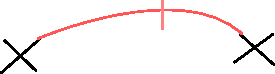
\includegraphics[width=0.3\linewidth]{brusselsproutend1}
		\end{center}
		\begin{center}
		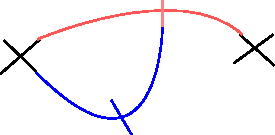
\includegraphics[width=0.3\linewidth]{brusselsproutend2}
		\end{center}
		\begin{center}
		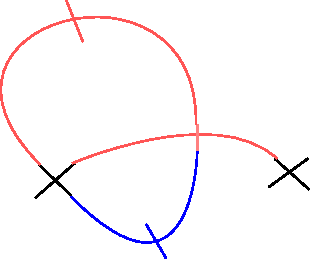
\includegraphics[width=0.3\linewidth]{brusselsproutend3}
		\end{center}
		\item The game ends when there is no more possible move. The player that draw the last valid line wins. Here is an example of the board at the end.
		\begin{center}
			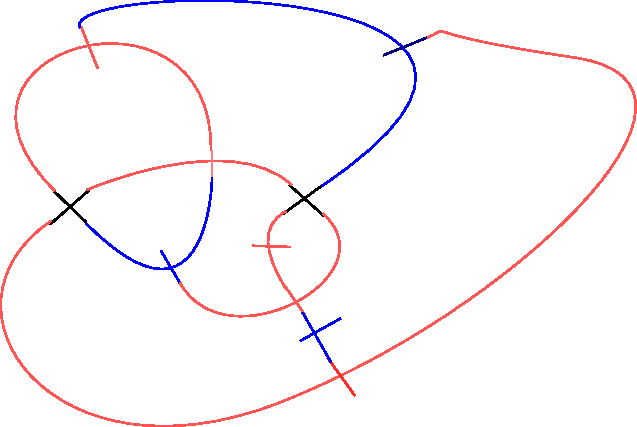
\includegraphics[width=0.7\linewidth]{brusselsproutend8}
		\end{center}
	\end{itemize}

	
	After playing this a few time, you will probably realize that not only that the second player always win. The game always end in exactly 8 turns. Let us this.
	
	\theorem The number of free end is always 8.
	
	\proof First, the number of free ends never change. Each time we draw a line we destroy to free end one for each end of the line. Then, we create two more by crossing the middle of a line. 
	
	Since we start with 8 free ends, we will always have 8 free ends.
	\qedd
	
	\theorem The game ends after exactly 8 turns.
	
	\proof Let assume that we are at turn $m$. Let us start by counting the number of vertex and edges.
	\begin{itemize}
	\item Since we start with 2 vertex and each time we draw a line we create one more vertex. Thus,
	\[
		v_m = 2+m.
	\]
	
	\item For the number of edges, since we start with 0 edge. At each turn we create two more edges (one left and one right of the newly created cross). Thus,
	\[
		e_m = 2m.
	\]
	
	\item Now we need the condition for the end of the game. The game ends when each face has exactly one free end in it. If it has more than one free end, then you can continue the game. So the condition for end of game is
	\[
		\text{\# faces} = \text{\# free end}
	\]
	
	\item We know from the previous theorem that the number of free end is always 8. This means that the game ends when we have $8$ faces.
	
	\item Now our job is to find the number of turn needed to create 8 faces. We can use euler formula for this
	\begin{align*}
		f + v = e+2
	\end{align*}
	That means at the end of the game where $f=8$ the turn number $m$  can be found from
	\[
		8 + (2 +m) = 2m + 2
	\]
	Solving for $m$ gives
	\[
		m = 8
	\]
	
	\item This means that the 8th turn is the last turn of the game. So the second player always win.
	\end{itemize}
	\qedd
	\section*{Matching Problem}
	\subsection*{Stable Marriage}
		Let us consider a situation where there are two married couple: (Alice, Bob) and (Charles, Dorothy). Let us suppose that Alice like Charles more than her husband Bob. Moreover, Charles like Alice more than his wife Dorothy. If this situation happens Alice and Charles are going to ditch their spouse and run off together. Such marriages are called unstable and Alice and Charles is called a rogue couple.
		
		Let us consider a village far away where there are equal number of boys and girl. You are a little cupid. Your job is to match boys and girls together such that there is no rogue couple. So, people in the village can live happily ever after.
		
	\subsubsection*{Mating Ritual}
		After a couple hour of deep thought. You came up with a mating ritual which goes like the following
		\begin{enumerate}
			\item First you have every boys ranks the girls according to his preference. The girls also make their list of boys according to her preference.
			
			\item On the first day, each girl wait at her balcony. Each boy then walk to his favorite girl on the list.
			\begin{itemize}
				\item Each girl then looks at all the boys at her balcony and pick her favorite.
				\item Each girl tells all the boys at her balcony that she did not pick to never come back again. The boy then cross the girl's name off his list.
				\item Each girl tells the boy she pick for that day to ``come back tomorrow and that she \emph{may} marry him.''
			\end{itemize}
			
			\item On the subsequent days the process is then repeated. Each boy go to his favorite girl that hasn't been crossed out yet. The girl then pick her favorite tell him to wait and tell everyone else to go away.
			
			\item The ritual ends when there is exactly one boy at each balcony.
		\end{enumerate}
		 
	\subsubsection*{Ritual Eventually Ends}
		
		First thing that probably come to our mind is that is this ritual a troll? We may get into an infinite loop. Actually, we are guarantee that the ritual will end after finite steps.
		
		The technique we use here is a general technique to show that some algorithm actually terminates. The idea is to monitor some finite resource and to show that the finite resource we have is strictly decreasing(at steady rate). Then we will run out of resource in finite number of step.
		
		The resource we are considering here is the number of girls on every boys list. If the ritual doesn't end yet, that means there is at one girl that has 2 or more boys at her balcony. This means one boy has to cross out a girl from his list. Since the number of girls on boys list is finite. The ritual will eventually end.
		
		You also know that everyone will get married at the end by pigeon hole. If there is empty balcony then there is at least one balcony with 2 boys which means the ritual doesn't end yet.
	
	\subsubsection*{Every Marriage is Stable}
	
		Another question you may ask is whether the pairing provide by this ritual is actually stable. We will prove this by showing that for any pair or boy and girl who are not married at the end of the ritual are not rogue couple.
		
		Let us consider Alice and Bob who are not married at the end of the ritual. There are two cases.
		
		\begin{itemize}
			\item Case 1. Alice is \emph{not} on Bob's list at the end. This means that Bob crossed Alice out on the day Alice found a better guy(Charles). Since we know that Alice must prefer her husband at least as much as Charles. We know that Alice must prefer her husband over Bob. So, Alice will never run away from her husband.
			
			\item Case 2. Alice is still on Bob's list at the end. This means that Bob is stuck with a girl whom he prefer over Alice. That means Bob prefer his wife over Alice. So, Bob will not run away from his wife. 
		\end{itemize}
		\qedd
		
	\subsubsection*{Life is Good for Boys}
	
	This ritual seem like a really good deal for girls. Afterall, the girls get to pick her favorite boys that comes to her balcony while the boys keeps getting rejected go home crying over and over again.
	
	To get and idea of who is getting a better deal. Let us consider 
	
	\definition \emph{Realm of possible Spouses} of a person A. Let us consider all possible stable matching on the preference list. Then we list all spouses of A on all those stable matching. Then the set is called realm of possible Spouses.
	
	Person A can also rank all spouses in his/her realm of possible Spouses. The one with the highest rank is the \emph{best possible spouse} and the one with the lowest rank is \emph{worst possible spouse}.
	
	\theorem The mating ritual marries every boy to his best possible spouse.
	
	\proof We will prove this by contradiction. Let us assume for the sake of contradictino that some boy doesn't not get married to his best possible spouse Alice.
	\begin{itemize}
		\item This means that there is the \emph{first} day where a boy cross out his best possible spouse. Let us call the boy (Bob) and the girl (Alice).
		
		\item Since Bob crosses out Alice that mean on that day Alice met someone better than Bob. Let us called that person Charles. So we know that
		\begin{center}
			Alice like Charles more than Bob.
		\end{center}
		
		\item Since this is the first day that anyone crosses out their best possible spouse. Charles has not cross out his best possible spouse (Dorothy) or in other words Charles has not visit his possible spouse. This means
		\begin{center}
			Charles likes Alice more than Dorothy.
		\end{center}
		
		\item Now since Alice is Bob's best possible spouse, there is a \emph{stable} marriage which Alice is married to Bob.
		
		However, in this stable marriage Charles will get matched with someone which he ranks at best as high as Dorothy since Dorothy is Charles' best possible spouse. This means Charles still likes Alice more than his wife.
		
		\item Since Alice like Charles more than her husband and Charles like Alice more than his wife. Charles and Alice are rogue couple in this stable marriage. Thus we have a contradiction.
		
		\item Therefore, in mating ritual, every boy gets married to his best possible spouse.
	\end{itemize}
	\qedd
	\subsubsection*{Not so much for Girl}
	
	\theorem The mating ritual marries every girl to her worst possible spouse.
	
	\proof Let us show this by contradiction. 
	\begin{itemize}
	\item Let us supposed that the mating ritual marries a girl (Alice) to someone (Bob) whom she likes more than her worst possible spouse(Charles). So we know that
	\begin{center}
		Alice likes Bob more than Charles.
	\end{center}
	
	\item From the previous theorem we know that Alice must be Bob's best possible spouse since the mating ritual match them together. This means
	\begin{center}
		Bob prefer Alice to everyone in realm of possible spouse.
	\end{center}
	
	\item Let us consider a stable marriage $M$\footnote{Not produced by the mating ritual.} where Alice is married to Charles. We know that such stable marriage exists since Charles is worst possible spouse for Alice. Thus
	\begin{center}
		In $M$, Alice is married to Charles whom she likes less than Bob.
	\end{center}
	
	\item In $M$, Bob has to be married to someone whom he like less than Alice since Alice is his possible spouse and Alice is already married to someone else.
	\begin{center}
		In $M$, Bob is married to someone whom he like less than Alice.
	\end{center}
	
	\item That means that in stable marriage $M$, Bob and Alice are rogue couple. Therefore, we have our contradiction.
	
	\item Thus, mating ritual marries every girl to her worst possible spouse. Poor girls. 
	
	\end{itemize}
	
	\qedd
	
	
	
	
	
	
	
	
	


	
	


\end{document}
